\documentclass[11pt]{article}
% Shared preamble of the RMC kernel write-ups (% Shared preamble of the RMC kernel write-ups (% Shared preamble of the RMC kernel write-ups (\input{preamble} after \documentclass).
\usepackage[margin=1in]{geometry}
\usepackage{amsmath,amssymb,bm}
\usepackage{graphicx}
\usepackage{booktabs}
\usepackage{hyperref}

\newcommand{\dd}{\,\mathrm{d}}
\newcommand{\Ein}{E}
\newcommand{\Eout}{E'}
\newcommand{\Ecm}{E_{c}}
\newcommand{\mucm}{\mu_{c}}
\newcommand{\mulab}{\mu_0}

% Common closing section: how the verification figures are produced
\newcommand{\verificationmethod}{%
Each figure is produced by \texttt{verification/verify\_laws.py}. For an incident
energy $\Ein$ along $+z$, $10^6$ collisions are sampled with MC/DC's own reaction
sampler (\texttt{sample\_elastic\_scattering}, \texttt{sample\_inelastic\_scattering}
or \texttt{sample\_fission}), and every emitted neutron is histogrammed in
$48 \times 24$ bins of $(\Eout, \mulab)$, with $\mulab$ the lab cosine to $+z$. The
inverted kernel used by RMC is integrated over the same bins (Gauss--Legendre panels;
two-body lines are split where $\mulab^*(\Eout)$ crosses a cosine edge), multiplied by
the number of collisions, and compared with a $\chi^2$ test over bins with at least 5
expected counts (the rest pooled into one bin). The tables list $\chi^2/\mathrm{dof}$,
its $p$-value, the emitted neutrons per collision (sampled vs.\ the integral of the
inverted kernel), and the largest relative change of a bin integral when the
quadrature panels are doubled. Left panels: outgoing-energy marginal; middle:
lab-cosine marginal; right: per-bin $z = (\text{sampled} - \text{inverted}) /
\sqrt{\text{inverted}}$.}
 after \documentclass).
\usepackage[margin=1in]{geometry}
\usepackage{amsmath,amssymb,bm}
\usepackage{graphicx}
\usepackage{booktabs}
\usepackage{hyperref}

\newcommand{\dd}{\,\mathrm{d}}
\newcommand{\Ein}{E}
\newcommand{\Eout}{E'}
\newcommand{\Ecm}{E_{c}}
\newcommand{\mucm}{\mu_{c}}
\newcommand{\mulab}{\mu_0}

% Common closing section: how the verification figures are produced
\newcommand{\verificationmethod}{%
Each figure is produced by \texttt{verification/verify\_laws.py}. For an incident
energy $\Ein$ along $+z$, $10^6$ collisions are sampled with MC/DC's own reaction
sampler (\texttt{sample\_elastic\_scattering}, \texttt{sample\_inelastic\_scattering}
or \texttt{sample\_fission}), and every emitted neutron is histogrammed in
$48 \times 24$ bins of $(\Eout, \mulab)$, with $\mulab$ the lab cosine to $+z$. The
inverted kernel used by RMC is integrated over the same bins (Gauss--Legendre panels;
two-body lines are split where $\mulab^*(\Eout)$ crosses a cosine edge), multiplied by
the number of collisions, and compared with a $\chi^2$ test over bins with at least 5
expected counts (the rest pooled into one bin). The tables list $\chi^2/\mathrm{dof}$,
its $p$-value, the emitted neutrons per collision (sampled vs.\ the integral of the
inverted kernel), and the largest relative change of a bin integral when the
quadrature panels are doubled. Left panels: outgoing-energy marginal; middle:
lab-cosine marginal; right: per-bin $z = (\text{sampled} - \text{inverted}) /
\sqrt{\text{inverted}}$.}
 after \documentclass).
\usepackage[margin=1in]{geometry}
\usepackage{amsmath,amssymb,bm}
\usepackage{graphicx}
\usepackage{booktabs}
\usepackage{hyperref}

\newcommand{\dd}{\,\mathrm{d}}
\newcommand{\Ein}{E}
\newcommand{\Eout}{E'}
\newcommand{\Ecm}{E_{c}}
\newcommand{\mucm}{\mu_{c}}
\newcommand{\mulab}{\mu_0}

% Common closing section: how the verification figures are produced
\newcommand{\verificationmethod}{%
Each figure is produced by \texttt{verification/verify\_laws.py}. For an incident
energy $\Ein$ along $+z$, $10^6$ collisions are sampled with MC/DC's own reaction
sampler (\texttt{sample\_elastic\_scattering}, \texttt{sample\_inelastic\_scattering}
or \texttt{sample\_fission}), and every emitted neutron is histogrammed in
$48 \times 24$ bins of $(\Eout, \mulab)$, with $\mulab$ the lab cosine to $+z$. The
inverted kernel used by RMC is integrated over the same bins (Gauss--Legendre panels;
two-body lines are split where $\mulab^*(\Eout)$ crosses a cosine edge), multiplied by
the number of collisions, and compared with a $\chi^2$ test over bins with at least 5
expected counts (the rest pooled into one bin). The tables list $\chi^2/\mathrm{dof}$,
its $p$-value, the emitted neutrons per collision (sampled vs.\ the integral of the
inverted kernel), and the largest relative change of a bin integral when the
quadrature panels are doubled. Left panels: outgoing-energy marginal; middle:
lab-cosine marginal; right: per-bin $z = (\text{sampled} - \text{inverted}) /
\sqrt{\text{inverted}}$.}


\title{Inverted kernel: tabulated energy--angle distribution (ACE Law 61)}
\date{}

\begin{document}
\maketitle

\noindent Code: \texttt{evaluate\_tabulated\_energy\_angle},
\texttt{correlated\_energy\_breakpoints},
\texttt{tabulated\_energy\_angle\_cosine\_breakpoints} in \texttt{mcdc/rmc/evaluate.py}.

\section{What MC/DC samples}

\noindent Source: \acespec{4.3.11.12}. Law 61 is an ACE identifier; ENDF's
correlated continuum data use MF=6 representations. The nearest-CDF angular
table rule below documents MC/DC's sampler, rather than continuous interpolation
of a physical angular density.

\texttt{sample\_tabulated\_energy\_angle}: incident grid $E_l$, outgoing tables
$\{E'_{l,k}, p_{l,k}, c_{l,k}\}$ (linear PDFs), and for every outgoing point $k$ an
angular table $\{\mu_{k,n}, q_{k,n}\}$ (linear PDF).
\begin{enumerate}
  \item The outgoing energy exactly as for Kalbach--Mann
  (\texttt{kalbach\_mann.tex}): table $l = i$ or $i+1$ with probabilities $1-f$, $f$,
  $\hat E$ by inversion of the linear PDF on interval $k$ for a random number $\xi_2$,
  and unit-base scaling to $\Eout$.
  \item The angular table of the outgoing point \emph{nearest in CDF}: table $k+1$ if
  $\xi_2 - c_{l,k} > c_{l,k+1} - \xi_2$, otherwise table $k$; then $\mu$ from that
  table by exact inversion.
\end{enumerate}

\section{Inverted kernel}

With $\hat E_l(\Eout)$, its interval $k$, $\Delta = \hat E_l - E'_{l,k}$ and slope
$m = (p_{l,k+1} - p_{l,k})/(E'_{l,k+1} - E'_{l,k})$, the random number that produced
$\hat E_l$ is its CDF value
\begin{equation}
  \hat c = c_{l,k} + p_{l,k}\Delta + \tfrac12 m\Delta^2 ,
\end{equation}
so the angular table is $n(\hat E_l) = k+1$ if $\hat c - c_{l,k} > c_{l,k+1} - \hat c$
and $k$ otherwise. The joint density is
\begin{equation}
  f(\Eout, \mu \mid \Ein) = \sum_{l \in \{i, i+1\}} w_l\;
  p_l(\hat E_l)\,\frac{E'_{l,K_l} - E'_{l,1}}{E'_{\max} - E'_{\min}}\;
  q_{l,n(\hat E_l)}(\mu),
\end{equation}
with $q_{l,n}$ the linear angular PDF of outgoing point $n$ in incident table $l$.
The table switch makes the angular
density jump where $\hat c$ crosses the CDF midpoint of an interval; solving
$c_{l,k} + p_{l,k}\Delta + \tfrac12 m\Delta^2 = c_{l,k} + \tfrac12(c_{l,k+1} - c_{l,k})$,
\begin{equation}
  \Delta_{1/2} = \frac{\sqrt{p_{l,k}^2 + m\,(c_{l,k+1} - c_{l,k})} - p_{l,k}}{m}
  \quad (m \ne 0),\qquad \Delta_{1/2} = \frac{c_{l,k+1}-c_{l,k}}{2p_{l,k}}\quad (m = 0),
\end{equation}
and these points (scaled to $\Eout$) are quadrature breakpoints, as are the cosine
grid points of the selected angular tables. In the COM frame
$f_L = Y f(\Ecm, \mucm)\sqrt{\Eout/\Ecm}$.

\section{Verification}
\verificationmethod

\begin{center}
\begin{tabular}{rrrrrrr}
\toprule
$E$ [eV] & samples & bins & $\chi^2/\mathrm{dof}$ & $p$ & yield (sampled / inverted) & quad. err. \\
\midrule
1e+07 & 1e+06 & 795 & 787.6/795 & 0.568 & 1.00000 / 1.00000 & 1.3e-04 \\
1.8e+07 & 1e+06 & 723 & 757.8/723 & 0.179 & 1.00000 / 1.00000 & 1.6e-04 \\
\bottomrule
\end{tabular}

\end{center}

\begin{figure}[h]
  \centering
  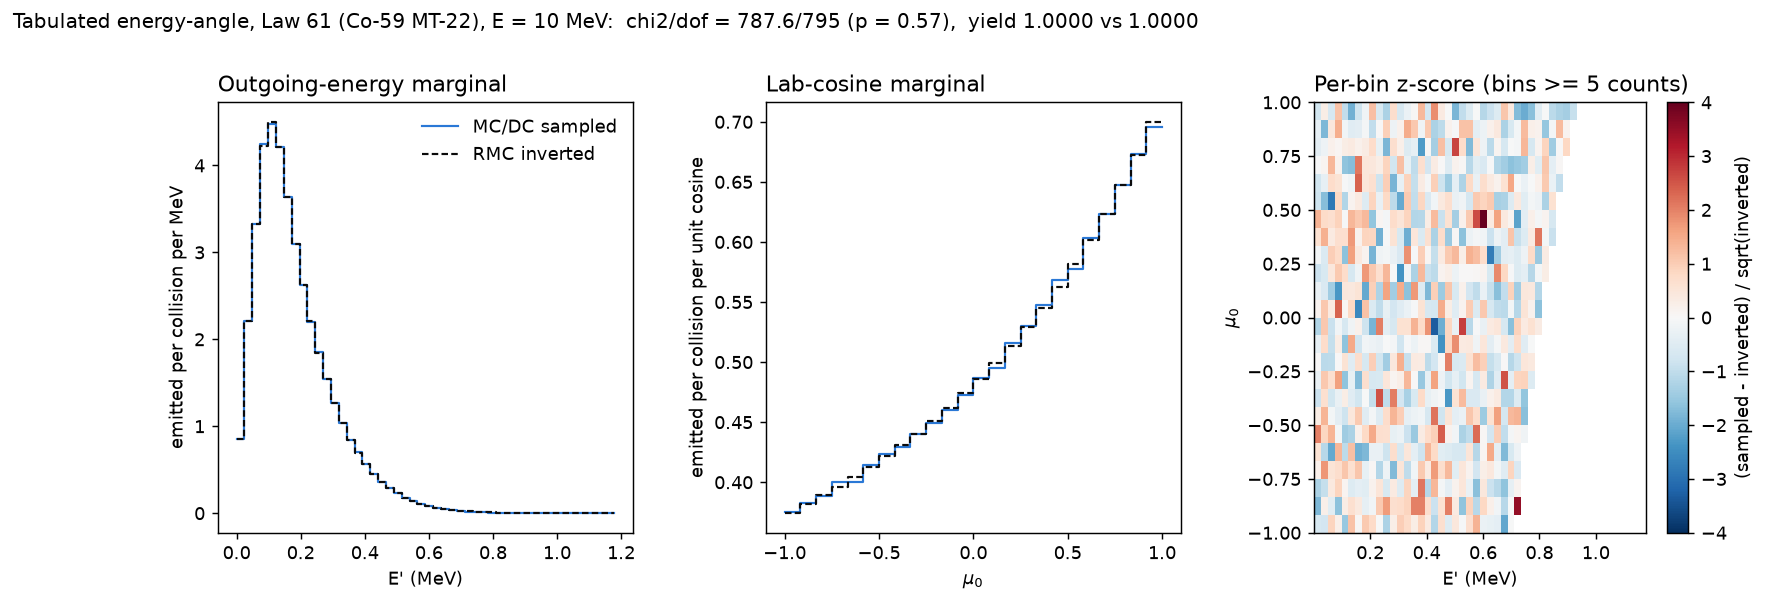
\includegraphics[width=\textwidth]{figures/energy_angle/energy_angle_E1e07.png}
  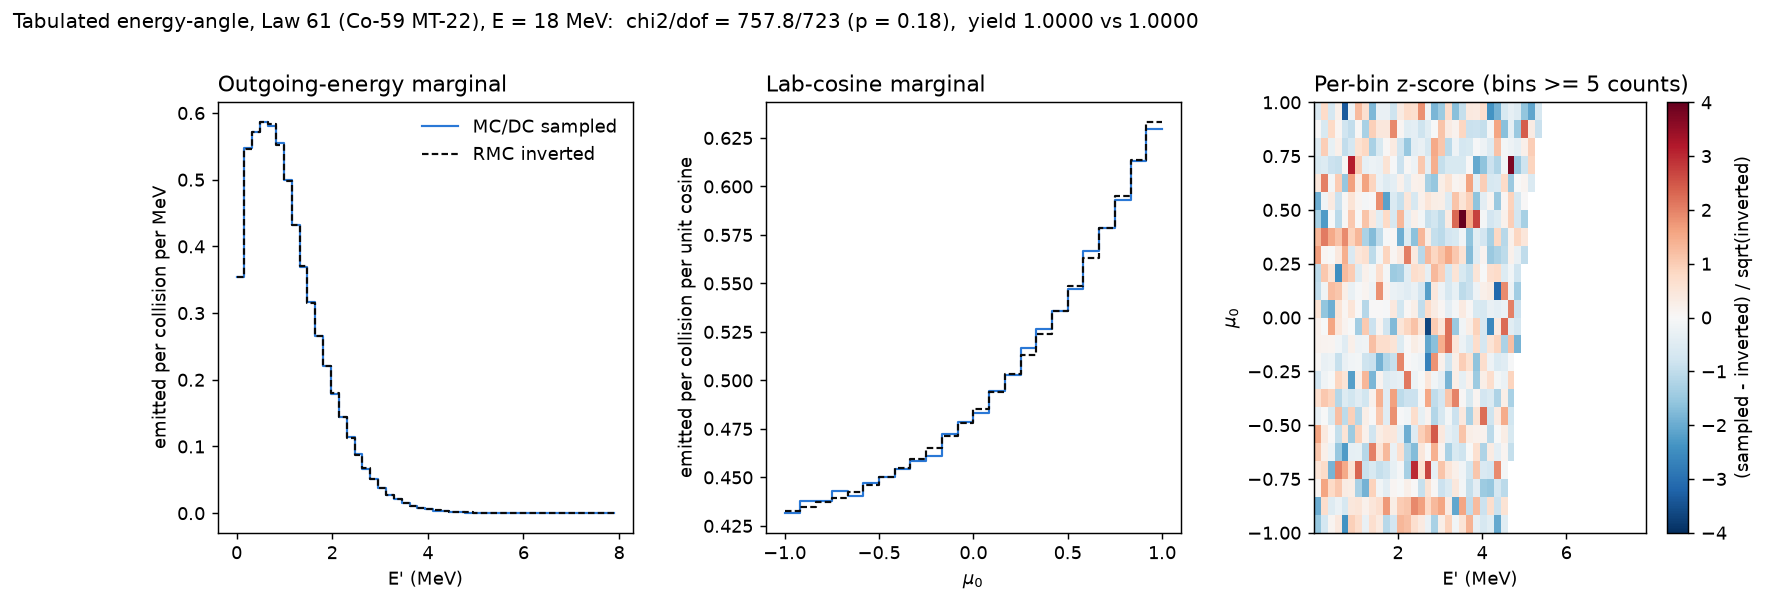
\includegraphics[width=\textwidth]{figures/energy_angle/energy_angle_E1p8e07.png}
  \caption{Co-59 MT-22 $(n,n\alpha)$, Law 61 in the COM frame, at 10 and 18\,MeV.}
\end{figure}

\end{document}
